\documentclass[12pt,floatfix,reprint,nofootinbib,amsmath,amssymb,epsfig,pre,floats,letterpaper,groupedaffiliation]{revtex4-1}

\usepackage{amsmath}
\usepackage{amssymb}
\usepackage{amsthm}
\usepackage{bm}
\usepackage{dcolumn}
\usepackage[english]{babel}
\usepackage{enumitem}
\usepackage{epstopdf}
\usepackage{graphicx}
\usepackage{hyperref}
\usepackage{inconsolata}
\usepackage{listings}
\usepackage{xcolor}
\usepackage{footmisc}
\usepackage{natbib}
\usepackage{url}
\usepackage{titlesec}
\usepackage{indentfirst}
\usepackage{inconsolata}
\usepackage[left=0.7in, right=0.66in, top=53pt]{geometry} % Adjust the margins
\usepackage{microtype}
\microtypesetup{protrusion=true, expansion=true, activate={true,nocompatibility}, final}

\newcommand{\beq}{\begin{equation}}
\newcommand{\eeq}{\end{equation}}
\newcommand{\e}{\mathrm{e}}
\newcommand{\la}{\langle}
\newcommand{\ra}{\rangle}

\newtheorem{theorem}{Theorem}
\newtheorem{lemma}[theorem]{Lemma}
\newtheorem{assumption}{Assumption}

\theoremstyle{definition}
\newtheorem{observation}{Observation}

\theoremstyle{definition}
\newtheorem{definition}{Definition}

\titlespacing{\subsection}{0pt}{24pt}{14pt plus 1pt}
\titlespacing*{\subsubsection}{0pt}{22pt plus 12pt minus 12pt}{15pt}
\linespread{0.928}
\setlength{\skip\footins}{34pt plus 34pt minus 12pt}
\interfootnotelinepenalty=10000
\setlength{\parskip}{2pt}
\interlinepenalty=0
\hyphenpenalty=0

\usepackage{etoolbox}
\AtBeginDocument{
  \setlength{\abovedisplayskip}{10pt}
  \setlength{\belowdisplayskip}{10pt}
  \setlength{\abovedisplayshortskip}{-4pt}
  \setlength{\belowdisplayshortskip}{6pt}
}

\begin{document}

\flushbottom


\title{Augur: a Decentralized Oracle and Prediction Market Platform}

\author{Jack Peterson}
\author{Joseph Krug}
\author{Ryan Garner}
\author{Micah Zoltu}
\author{Austin K. Williams}
\author{Stephanie Alexander}
\affiliation{Forecast Foundation}
\date{July 12, 2018}

\begin{abstract}

\vspace{0pt plus 20pt}
Augur is a trustless, decentralized oracle and platform for prediction markets. The outcomes of Augur's prediction markets are chosen by users that hold Augur's native Reputation token, who stake their tokens on the actual observed outcome and, in return, receive settlement fees from the markets. Augur's incentive structure is designed to ensure that honest, accurate reporting of outcomes is always the most profitable option for Reputation token holders. Token holders can post progressively-larger Reputation bonds to dispute proposed market outcomes. If the size of these bonds reaches a certain threshold, Reputation splits into multiple versions, one for each possible outcome of the disputed market; token holders must then exchange their Reputation tokens for one of these versions. Versions of Reputation which do not correspond to the real-world outcome will become worthless, as no one will participate in prediction markets unless they are confident that the markets will resolve correctly. Therefore, token holders will select the only version of Reputation which they know will continue to have value: the version that corresponds to reality.
\end{abstract}

\maketitle

Augur is a trustless, decentralized oracle and predic-\linebreak tion market platform. In a prediction market, \mbox{individuals} can speculate on the outcomes of future events; those who\linebreak forecast the outcome correctly win money, and those who forecast incorrectly lose money~\cite{Wolfers_2004,Surowiecki_2005,Hanson_2006}. The price of a prediction market can serve as a precise and well-calibrated indicator of how likely an event is to occur~\cite{Pennock_2001,Manski_2004,Wolfers_2005,Goel_2010}.

Using Augur, people will have the ability to trade in prediction markets at very low cost. The only significant\linebreak expenses participants assume is compensation to mar-\linebreak ket creators and to users that report on the outcomes of markets once the event has taken place. The result is\linebreak a prediction market where trust requirements, friction,\linebreak and fees will be as low as competitive market forces can drive them.

Historically, prediction markets have been centralized. The simplest way to aggregate trades in a prediction mar-\linebreak ket is for a trustworthy entity to maintain a ledger; sim-\linebreak ilarly, the simplest way to determine the outcome of an event and distribute payouts to traders is for an impar-\linebreak tial, trusted judge to determine the outcomes of the mar-\linebreak kets. However, centralized prediction markets have many risks and limitations: they do not allow global participa-\linebreak tion, they limit what types of markets can be created or\linebreak traded, and they require traders to trust the market op-\linebreak erator to not steal funds and to resolve markets correctly.

Augur aims to resolve markets in a fully decentralized way. Decentralized, trustless networks, such as Bitcoin~\cite{Nakamoto_2008} and Ethereum~\cite{Buterin_2013}, eliminate the risk that self-interest will turn into corruption or theft. The only role of the Augur\linebreak developers is to publish smart contracts to the Ethereum network. The Augur contracts are totally automated:\linebreak the developers do not have the ability to spend funds\linebreak that are held in escrow on-contract, do not control how markets resolve, do not approve or reject trades or other transactions on the network, cannot undo trades, can-\linebreak not modify or cancel orders, etc. The Augur \textit{oracle} allows information to be migrated from the real world to\linebreak a blockchain without relying on a trusted intermediary. Augur will be the world's first decentralized oracle.

\section{HOW AUGUR WORKS}

\vspace{0pt plus 20pt}

Augur markets follow a four-stage progression: \textit{cre-\linebreak ation}, \textit{trading}, \textit{reporting}, and \textit{settlement}. Anyone can\linebreak create a market based on any real-world event. Trading\linebreak begins immediately after market creation, and all users\linebreak are free to trade on any market. After the event on which the market is based has occurred, the outcome of the\linebreak event is determined by Augur's oracle. Once the out-\linebreak come is determined, traders can close out their positions and collect their payouts.

\vspace{0pt plus 20pt}

Augur has a native token, Reputation (REP). REP is needed by market creators and by reporters when they report on the outcome of markets created on the Augur platform. Reporters report on a market by \textit{staking} their REP on one of the market's possible outcomes. By doing this, the reporter declares that the outcome on which the stake was placed matches the real-world outcome of the market's underlying event. The consensus of a market's reporters is considered the ``truth" for the purpose of determining the market's outcome. If a reporter's report of a market's outcome does not match the consensus reached by the other reporters, Augur redistributes the REP staked on the non-consensus outcome by this re-\linebreak porter to the reporters that reported with the consensus.

\vspace{0pt plus 20pt}

By owning REP, and participating in the accurate re-\linebreak porting on the outcomes of events, token holders are enti-\linebreak tled to a portion of the fees on the platform. Each staked REP token entitles its holder to an equal portion of Au-\linebreak gur's market fees. The more REP a reporter owns, and reports correctly with, the more fees they will earn for\linebreak their work in keeping the platform secure.

\vspace{0pt plus 20pt}

\begin{figure*}
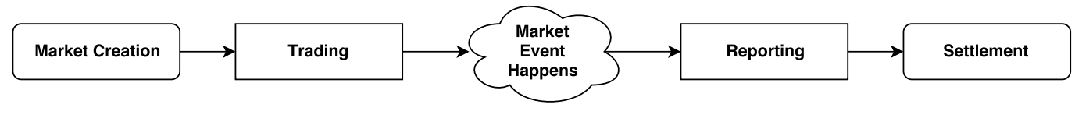
\includegraphics[width=0.82\textwidth]{1.pdf}
\caption{Simplified outline of the lifetime of a prediction market.}
\label{fig:overview}
\end{figure*}

Although REP plays a central role in Augur's opera-\linebreak tions, it is not used to trade in Augur's markets. Traders will never need to own or use REP, as they are not re-\linebreak quired to participate in the reporting process.\pagebreak



\subsection{Market Creation}

Augur allows anyone to create a market about any upcoming event. The \textit{market creator} sets the \textit{event end time} and chooses a \textit{designated reporter} to report the outcome of the event. The designated reporter does not unilat-\linebreak erally decide the outcome of the market; the community\linebreak always has an opportunity to dispute and correct the\linebreak designated reporter's report.

Next, the market creator chooses a \textit{resolution source} that reporters should use to determine the outcome. The resolution source may simply be ``common knowledge",\linebreak or it may be a specific source, such as ``The United States Department of Energy", \texttt{bbc.com}, or the address of a\linebreak particular API endpoint.\footnote{For example, if a market on ``The high tempera-\linebreak ture (in degrees Fahrenheit) on April 10, 2018 at the\linebreak San Francisco International Airport, as reported by\linebreak Weather Underground" specifies a resolution source of \url{https://www.wunderground.com/history/airport/KSFO/2018/4/10/DailyHistory.html}, reporters would simply go to that URL and enter the high temperature displayed there as their report.} They also set a \textit{creator fee}, which is the fee paid to the market creator by traders who settle with the market contract (see Section~\ref{section:settlement} for details on fees). Finally, the market creator posts two bonds:\linebreak the \textit{validity bond}, and the \textit{designated report no-show bond} (also referred to as the \textit{no-show bond} for brevity).

The validity bond is paid in ETH and is returned to the market creator if the market resolves to any out-\linebreak come other than \textit{invalid}.\footnote{An \textit{invalid market} is a market determined to be invalid by reporters because none of the outcomes listed by the market creator is cor-\linebreak rect, or because the market wording is ambiguous or subjective; see Section~\ref{section:ambiguous_or_subjective_markets} for discussion.} The validity bond incentivizes market creators to create markets based on well-defined events with objective, unambiguous outcomes. The size\linebreak of the validity bond is set dynamically, based on the pro-\linebreak portion of invalid outcomes in recent markets.\footnote{See Appendix~E.1 for details.}

{\spaceskip=1.07\fontdimen2\font plus 1pt minus 1pt
The no-show bond, paid in REP, is returned to the market creator if the market's designated reporter actually reports during the first three days after the market's \textit{event end time}. If the designated reporter does not submit their report during the allotted 3-day window, then the market creator forfeits the no-show bond and it\linebreak is given to the \textit{first public reporter} who reports on the market (see Section~I.C.6). This incentivizes the market\linebreak creator to choose a reliable designated reporter, which should help markets resolve quickly.} 

\vspace{\baselineskip}In the event that the designated reporter fails to re-\linebreak port, the no-show bond is given to the first public re-\linebreak porter in the form of stake on their reported outcome, so that the first public reporter receives the no-show bond if and only if they report correctly. As with the validity bond, the no-show bond is adjusted dynamically based\linebreak on the proportion of designated reporters who failed to report on time during the previous fee window.\footnote{See Appendix~E.2 for details.}

The market creator creates the market and posts all required bonds via a single Ethereum transaction. Once the transaction is confirmed, the market is live and trad-\linebreak ing begins.

\subsection{Trading}

Market participants forecast the outcomes of events by trading \textit{shares} of those market outcomes. A \textit{complete set of shares} is a collection of shares that consists of one share of each possible valid outcome of the event~\cite{Clark_2014}. Complete sets are created by Augur's on-contract matching engine as needed to complete trades.

For example, consider a market that has two possible outcomes, \texttt{A} and \texttt{B}. Alice is willing to pay 0.7 ETH for a share of \texttt{A} and Bob is willing to pay 0.3 ETH for a share of \texttt{B}.\footnote{Initially, trades in Augur's markets will use Ethereum's native coin, Ether (ETH). Subsequent releases of Augur will include support for markets denominated in arbitrary tokens issued on the Ethereum network, including shares of other markets as well as tokens pegged to fiat currencies (``stablecoins"), if/when these become available.} First, Augur matches these orders and collects a total of 1 ETH from Alice and Bob.\footnote{\label{footnote:complete_set_cost}The 1 ETH figure is used here for ease of discussion. The actual cost of a complete set of shares is much smaller than this; see \texttt{docs.augur.net/\#number-of-ticks} for details.} Then Augur creates a complete set of shares, giving Alice the share of \texttt{A} and Bob the share of \texttt{B}. This is how shares of outcomes come into existence. Once the shares are created, they can be traded freely.

The Augur trading contracts maintain an order book\linebreak for every market created on the platform. Anybody can create a new order or fill an existing order at any time. Orders are filled by an automated matching engine that exists within Augur's smart contracts. Requests to buy or sell shares are fulfilled immediately if there is a matching order already on the order book. It may be filled\linebreak by buying shares from or selling shares to other partic-\linebreak ipants, which, may involve issuing new complete sets or closing out existing complete sets. Augur's matching engine always sequesters the minimum amount of shares and/or cash needed to cover the value at risk. If there is no matching order, or the request can be only partially filled, the remainder is placed on the order book as a new order.

Orders are never executed at a worse price than the\linebreak limit price set by the trader, but may be executed at a better price. Unfilled and partially-filled orders can be removed from the order book by the order's creator at\linebreak any time. Fees are paid by traders only when complete sets of shares are sold; settlement fees are discussed in more detail in Section~\ref{section:settlement}.

While most trading of shares is expected to happen before market settlement, shares can be traded any time after market creation. All Augur assets -- including shares in market outcomes, participation tokens, shares in dis-\linebreak pute bonds, and even ownership of the markets them-\linebreak selves -- are transferable at all times.

\subsection{Reporting}

Once a market's underlying event occurs, the outcome must be determined in order for the market to finalize\linebreak and begin settlement. Outcomes are determined by Augur's oracle, which consists of profit-motivated reporters, who simply report the actual, real-world outcome of the event. Anyone who owns REP may participate in the reporting and disputing of outcomes. Reporters whose reports are consistent with consensus are financially rewarded, while those whose reports are not consistent with consensus are financially penalized (see Section I D 3).

\subsubsection{Fee Windows}

Augur's reporting system runs on a cycle of consecu-\linebreak tive 7-day long \textit{fee windows}. All fees collected by Augur during a given fee window are added to the \textit{reporting fee pool} for that fee window. At the end of the fee window, the reporting fee pool is paid out to REP holders who participated in the reporting process. Reporters receive rewards in proportion to the amount of REP they staked during that fee window. Participation includes: staking during an initial report, disputing a tentative outcome,\linebreak or purchasing \textit{participation tokens}.

\subsubsection{Participation Tokens}

During any fee window, REP holders may purchase any number of participation tokens for one attorep\footnote{One attorep is $10^{-18}$ REP.} each. At the end of the fee window, they may redeem their\linebreak \vspace{\baselineskip} participation tokens for one attorep each, in addition to a proportional share of the fee window's \textit{reporting fee pool}. If there were no actions (e.g., submitting a report or disputing a report submitted by another user) needed of a reporter, the reporter may purchase participation tokens to indicate that they showed up for the fee window. Just like staked REP, participation tokens may be redeemed by their owners for a pro rata portion of fees in this fee window.

As discussed in Section II, it is important that REP holders are ready to participate in market resolution in the event of a fork. The participation token provides an incentive for REP holders to monitor the platform at least once per week, and, thus, be ready to participate if the need arises. Even REP holders who do not want to participate in the reporting process are incentivized to check-in with Augur once per 7-day fee window in order to buy participation tokens and collect fees. This regular, active checking-in will ensure that they are familiar with how to use Augur, will be aware of forks when they occur, and thus should be more ready to participate in forks\linebreak when they happen.

\subsubsection{Market State Progression}

Augur markets can be in seven different states after creation. The potential states, or ``phases'', of an Augur market are as follows:

\begin{itemize}
\item Pre-reporting
\item Designated Reporting
\item Open Reporting
\item Waiting for the Next Fee Window to Begin
\item Dispute Round
\item Fork
\item Finalized
\end{itemize}

The relationship between these states can be seen in Fig.~2.

\subsubsection{Pre-reporting}

\begin{figure*}
    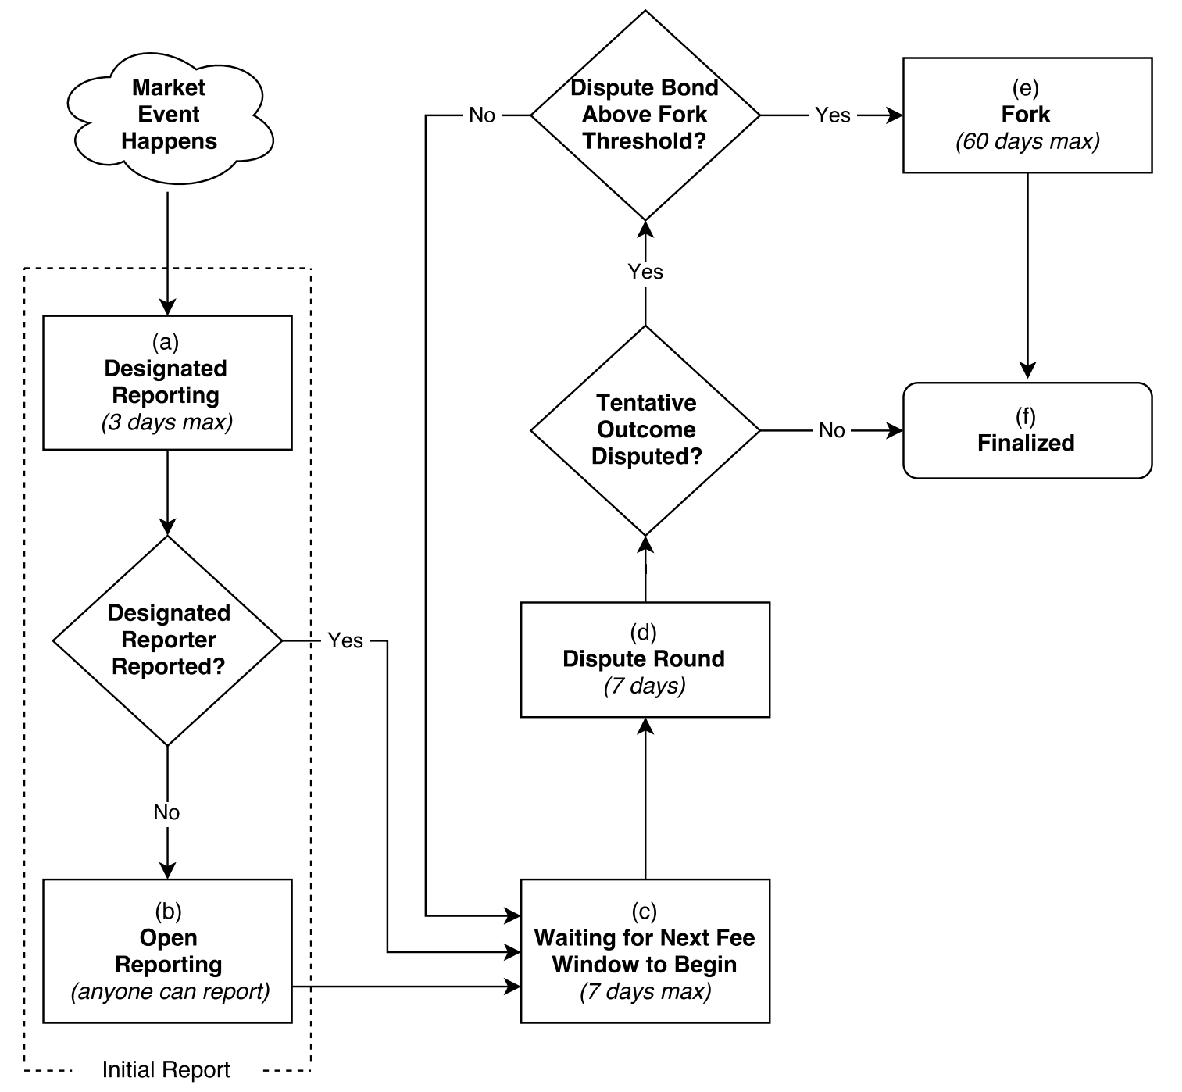
\includegraphics[width=0.805\textwidth]{2.pdf}
    \caption{Reporting flowchart.}
    \label{fig:reporting}
\end{figure*}

The \textit{pre-reporting} or \textit{trading} phase (Fig.~1) is the time period that begins after trading has begun in the market, but before the market's event has come to pass. Gener-\linebreak ally, this is the most active trading period for any given\linebreak Augur market. Once the event end date has passed, the market enters the \textit{designated reporting} phase (Fig.~2a).

\subsubsection{Designated Reporting}

When creating a market, market creators are required\linebreak to choose a designated reporter and post a no-show bond. During the designated reporting phase (Fig.~2a) the market's designated reporter has up to three days to report\linebreak on the outcome of the event. If the designated reporter fails to report within the allotted three days, the market creator forfeits the no-show bond, and the market automatically enters the \textit{open reporting} phase (Fig.~2b).

If the designated reporter submits a report on time, then the no-show bond is returned to the market creator.\linebreak The designated reporter is required to post the desig-\linebreak nated reporter stake\footnote{See appendix E 3 for details on the size of the designated reporter stake.} on its reported outcome, which it\linebreak will forfeit if the market finalizes to any outcome other\linebreak than the one they reported.\footnote{Forfeited stake is added to the reporting fee pool of the market's assigned fee window, and is used to reward honest reporters and disputers; see Section I D 3 for details.} As soon as the designated reporter submits its report, the market enters the \textit{waiting\linebreak for next fee window to begin} phase (Fig.~2c), and the re-\linebreak ported outcome becomes the market's \textit{tentative outcome}.

\subsubsection{Open Reporting}

If the designated reporter fails to report within the\linebreak allotted three days, the market creator forfeits the no-show bond, and the market immediately enters the \textit{open reporting} phase (Fig.~2b). As soon as the market enters the open reporting phase, anyone can report the outcome of the market. When the designated reporter fails to\pagebreak \linebreak report, the first reporter who reports on the outcome of\linebreak a market is called the market's \textit{first public reporter}.

The market's first public reporter receives the forfeited no-show bond in the form of stake on their chosen out-\linebreak come, so they may claim the no-show bond only if their reported outcome agrees with the market's final outcome. The first public reporter does not need to stake any of their own REP when reporting the outcome of the mar-\linebreak ket. In this way, any market whose designated reporter fails to report is expected to have its outcome reported by \textit{someone} very soon after entering the open reporting phase.

Once an \textit{initial report} has been received by the ini-\linebreak tial reporter (whether it was the designated reporter or first public reporter), the reported outcome becomes the market's tentative outcome, and the market enters the \textit{waiting for next fee window to begin} phase (Fig.~2c).

\subsubsection{Waiting for Next Fee Window to Begin}

Once the market receives its initial report, it enters the waiting for next fee window to begin phase (Fig.~2c). During this phase, reporting for the market is on hold un-\linebreak til end of the current fee window. Once the next fee win-\linebreak dow begins, the market enters the \textit{dispute round} phase.

\subsubsection{Dispute Round}

The dispute round (Fig.~2d) is a 7-day period during which any REP holder has the opportunity to dispute the market's \textit{tentative outcome}.\footnote{The fact that the dispute rounds coincide with the fee windows is purely a matter of convenience; in principle, dispute rounds and\linebreak fee window durations could be different.} (At the beginning of a dispute round, a market's tentative outcome is the out-\linebreak come that will become the market's final outcome if it\linebreak is not successfully disputed by REP holders.) A dispute consists of \textit{staking} REP (referred to as \textit{dispute stake} in\linebreak this context) on an outcome \textit{other than} the market's current tentative outcome. A dispute is \textit{successful} if the to-\linebreak tal amount of dispute stake on some outcome meets the \textit{dispute bond size} required for the current round. The dispute bond size is computed as follows.

Let $A_n$ denote the total stake over all of this market's outcomes at the beginning of dispute round $n$. Let $\omega$\linebreak be any market outcome \textit{other than} the market's tenta-\linebreak tive outcome at the beginning of this dispute round. Let $S(\omega, n)$ denote the total amount of stake on outcome $\omega$ at the beginning of dispute round $n$. Then the size of the \textit{dispute bond} needed to successfully dispute the current tentative outcome in favor of the new outcome $\omega$ during round $n$ is denoted $B(\omega, n)$ and is given by:

\beq
B(\omega, n) = 2A_n - 3S(\omega, n)
\eeq

The bond sizes are chosen this way to ensure a fixed ROI of 50\% for reporters who successfully dispute false outcomes (see Section II D).

The dispute bonds need not be paid in their entirety by a single user. The Augur platform allows participants to crowdsource dispute bonds. Any user who sees an incorrect tentative outcome can dispute that outcome by staking REP on an outcome other than the tentative outcome. If any outcome (other than the tentative outcome) accumulates enough dispute stake to fill its dispute bond, the current tentative outcome will be successfully dis-\linebreak puted.

In the case of a successful dispute, the market will\linebreak either undergo another dispute round, or it will enter\linebreak the \textit{fork} state (Fig.~2e). If the size of the filled dispute bond is greater than 2.5\% of all REP, then the market will enter the fork state. If the size of the filled dispute bond is less than 2.5\% of all REP, then the newly chosen outcome becomes the market's new tentative outcome, and the market undergoes another dispute round.

All dispute stake is held in escrow during the dispute round. If a dispute bond is unsuccessful, then the dis-\linebreak pute stake is returned to its owners at the end of the dispute round. If no dispute is successful during the 7-day dispute round, the market enters the \textit{finalized} state (Fig.~2f), and its tentative outcome is accepted as its \textit{fi\linebreak nal outcome}. A market's final outcome is the tentative outcome that passes through a dispute round without being successfully disputed, or is determined via a fork. Augur's contracts treat final outcomes as \textit{truth} and pay out accordingly.

All unsuccessful dispute stake is returned to the origi-\linebreak nal owners at the end of every dispute round. All success-\linebreak ful dispute stake is applied to the outcome it championed, and remains there until the market is finalized (or until a fork occurs in some other Augur market). All dispute stake (whether successful or unsuccessful) will receive a portion of the reporting fee pool\footnote{Any reporting fees and validity bonds collected during a fee window get added to that fee window's reporting fee pool. At the end of the fee window, the reporting fee pool is paid out to users in proportion to the amount of REP they staked during that fee window.} from the current fee window.

\subsubsection{Fork}

The fork state (Fig.~2e) is a special state that lasts up to 60 days. Forking is the market resolution method of last resort; it is a very disruptive process and is intended to be a rare occurrence. A fork is caused when there is a market with an outcome with a successfully-filled dispute bond of at least 2.5\% of all REP. This market is referred to as the \textit{forking market}\pagebreak.

When a fork is initiated, a 60-day\footnote{Forking periods can be less than 60 days: a forking period ends\linebreak when either 60 days have passed, or more than 50\% of all genesis REP is migrated to some child universe.} \textit{forking period} be-\linebreak gins. Disputing for all other non-finalized markets is put on hold until the end of this forking period. The forking period is much longer than the usual fee window because the platform needs to provide ample time for REP hold-\linebreak ers and service providers (such as wallets and exchanges)\linebreak to prepare. A fork's final outcome cannot be disputed.

Every Augur market and all REP tokens exist in some\linebreak \textit{universe}. REP tokens can be used to report on outcomes (and thus earn fees) \textit{only} for markets that exist in the\linebreak same universe as the REP tokens. When Augur first launches, all markets and all REP will exist together in the \textit{genesis universe}.

When a market forks, new universes are created. Forking creates a new \textit{child universe} for each possible out-\linebreak come of the forking market (including \texttt{Invalid}, as dis-\linebreak cussed in Section I D 2). For example, a ``Yes/No'' market has 3 possible outcomes: \texttt{Yes}, \texttt{No}, and \texttt{Invalid}. Thus, a ``Yes/No'' forking market will create three new child universes: universe \texttt{Yes}, universe \texttt{No}, and universe \texttt{Invalid}. Initially, these newly created universes are empty: they contain no markets or REP tokens.

When a fork is initiated, the \textit{parent universe} becomes permanently \textit{locked}. In a locked universe, no new markets may be created. Users may continue trading shares in markets in locked universes, and markets in a locked universe may still receive their initial reports. However, no reporting rewards are paid out there, and markets in locked universes cannot be finalized. In order for markets or REP tokens in the locked universe to be useful, they must first be migrated to a child universe.

Holders of REP tokens in the parent universe may migrate their tokens to a child universe of their choice. This choice should be considered carefully, because migration is one-way; it cannot be reversed. Tokens cannot be sent from one sibling universe to another. \textit{Migration is a permanent commitment of REP tokens to a particular mar-\linebreak ket outcome}. REP tokens that migrate to different child universes ought to be considered entirely separate tokens, and service providers like wallets and exchanges ought to list them as such.

When a fork is initiated, all REP staked on all non-forking markets is \textit{unstaked} so that it is free to be mi-\linebreak grated to a child universe during the forking period.\footnote{The only exception is the REP staked by the initial reporter when they made the initial report. That REP remains staked on the\linebreak initial reported outcome and is automatically migrated to the child universe that wins the fork.}

Whichever child universe receives the most migrated REP by the end of the forking period becomes the \textit{win-\linebreak ning universe}, and its corresponding outcome becomes\linebreak the final outcome of the forking market. Un-finalized\linebreak\vspace{\baselineskip}\vspace{0.3336\baselineskip}markets in the parent universe may be migrated only to\break\break the winning universe and, if they have received an initial report, are reset back to the waiting for next fee window to begin phase.

\textit{There is no time limit to migrate tokens from the par-\linebreak ent universe to a child universe.} Tokens may be mi-\linebreak grated after the forking period, but they will not count towards the determination of the winning universe. To\linebreak encourage greater participation during the forking pe-\linebreak riod, all token holders who migrate their REP within 60 days of the start of a fork will receive 5\% additional REP\linebreak in the child universe to which they migrated\footnote{This occurs even when the forking period has ended early due to more than 50\% of all REP being migrated to some child universe.}. This re-\linebreak ward is paid for by minting new REP tokens.\footnote{The effect of this addition to the money supply of REP is small. For example, if 20\% of all existing REP is migrated during the forking period of a fork, this bonus would result in a 1\% increase in the money supply of REP. Moreover, forks are expected to be exceedingly rare events.}

\textit{Reporters that have staked REP on one of the forking\linebreak market's outcomes cannot change their position during a\linebreak fork.} REP that was staked on an outcome in the par-\linebreak ent universe can be migrated only to the child universe that corresponds to that outcome. For example, if a re-\linebreak porter helped fulfill a successful dispute bond in favor\linebreak of outcome \texttt{A} during some dispute round, then the REP they have staked on outcome \texttt{A} can only be migrated to universe \texttt{A} during a fork.

\textit{Sibling universes are entirely disjoint.} REP tokens\linebreak that exist in one universe cannot be used to report on events or earn rewards from markets in another universe. Since users presumably will not want to create or trade on\linebreak markets in a universe whose oracle is untrustworthy, REP that exists in a universe that does not correspond to objective reality is unlikely to earn its owner any fees, and therefore should not hold any significant market value. Therefore, REP tokens migrated to a universe which does not correspond to objective reality should hold no market value, regardless of whether or not the objectively false universe ends up being the winning universe after\linebreak a fork. This has important security consequences, which we discuss in Section II.

\subsubsection{Finalized}

A market enters the finalized state (Fig.~2f) if it passes through a 7-day dispute round without having its tenta-\linebreak tive outcome successfully disputed, or after completion of\linebreak a fork. The outcome of a fork cannot be disputed and is always considered final at the end of the forking period. Once a market is finalized, traders can settle their po-\linebreak sitions directly with the market. When a market enters the finalized state, we refer to its chosen outcome as the \textit{final outcome}.

\subsection{Market Settlement}\label{section:settlement}

A trader can close their position in one of two ways: by selling the shares they hold to another trader in exchange for currency, or by settling their shares with the market. Recall that every share comes into existence as part of a complete set when a total of 1 ETH has been escrowed with Augur.\footref{footnote:complete_set_cost} To get that 1 ETH out of escrow, traders must give Augur either a complete set or, if the market has finalized, a share of the winning outcome. When this exchange happens we say traders are \textit{settling with the market contract}.

For example, consider a non-finalized market with pos-\linebreak sible outcomes \texttt{A} and \texttt{B}. Suppose Alice has a share of out-\linebreak come \texttt{A} that she wants to sell for 0.7 ETH and Bob has a share of outcome \texttt{B} that he wants to sell for 0.3 ETH. First, Augur matches these orders and collects the \texttt{A} and\linebreak \texttt{B} shares from the participants. Then Augur gives 0.7\linebreak ETH (minus fees) to Alice and 0.3 ETH (minus fees) to\linebreak Bob.

As a second example, consider a finalized market whose winning outcome is \texttt{A}. Alice has a share of \texttt{A} and wants to cash it in. She sends her share of \texttt{A} to Augur and in return receives 1 ETH (minus fees).

\subsubsection{Settlement Fees}

The only time Augur levies fees is when market par-\linebreak ticipants are settling with the market contract. Augur levies two fees during settlement: the creator fee, and\linebreak the reporting fee. Both of these fees are proportional to the amount being paid out. So, in the pre-finalized settlement example above, where Alice receives 0.7 ETH and Bob receives 0.3 ETH, Alice would pay 70\% of the fees while Bob would pay 30\%.

The creator fee is set by the market creator during market creation, and is paid to the market creator upon settlement. The reporting fee is set dynamically (see Sec-\linebreak tion~\ref{section:market_cap_nudges}) and is paid to reporters who participate in the reporting process.

\subsubsection{Settlement of Invalid Markets}

In the event that a market resolves as \texttt{Invalid}, traders who settle with the market contract receive an equal amount of ETH for shares of each outcome. If the market had $N$ possible outcomes (not including the \texttt{Invalid} outcome), and the cost of a complete set of shares was $C$ ETH, then traders will receive $C/N$ ETH for each share settled with the market contract.
\footnote{Trades cannot simply be unwound if a market resolves as Invalid\linebreak due to technical limitations. Shares of outcomes are just tokens, which can be traded directly between users; the ETH and shares are thus not under Augur's control and cannot be given back to the original owner if the market finalizes as Invalid.}

\subsubsection{Reputation Redistribution}\label{section:rep_redistribution}

If a market finalizes without initiating a fork, all REP staked on any outcome other than the market's final\linebreak outcome is forfeited and distributed to the users who staked on the market's final outcome in proportion to\linebreak the amount of REP they staked. The dispute bond sizes are chosen such that anyone who successfully disputes\linebreak an outcome in favor of the market's final outcome is rewarded with a 50\% ROI on their dispute stake.\footnote{See Theorem~3 in Appendix~A.} This is a strong incentive for reporters to dispute false tentative outcomes.

\section{Incentives and Security}\label{section:incentives_and_security}

There is a strong relationship between the market cap of REP and the trustworthiness of Augur's forking proto-\linebreak col. If the market cap of REP is large enough\footnote{See Section~\ref{section:integrity_forking_protocol} for details.}, and at-\linebreak tackers are economically rational, then the outcome that wins the fork should correspond to objective reality. In fact, it would be possible for Augur to function properly without using designated reporters and dispute rounds. Using \textit{only} the forking process, the oracle would report truthfully.

However, forks are disruptive and time consuming. A fork takes up to 60 days to resolve a single market, and can resolve only one market at a time. During the 60 days in which the forking market is being resolved, all\linebreak other non-finalized markets are put on hold.\footnote{Traders can continue trading on those markets, but those markets cannot finalize until after the forking period.} Service providers have to update, and REP holders have to migrate their REP to one of the new child universes. Therefore, forks should be used only when they are absolutely necessary. Forking is the nuclear option.

Fortunately, once it has been established that forks can be trusted to determine truth, incentives can be used to encourage participants to behave honestly without hav-\linebreak ing to actually initiate a fork. \textit{It is the credible threat of\linebreak a fork, and the belief that the fork will resolve correctly,\linebreak that are the cornerstones of Augur's incentive system.}

Next, we discuss the conditions under which the fork-\linebreak ing system can be trusted to determine truth. We then discuss the incentive system and how it encourages quick and correct resolution of all markets.

\subsection{Integrity of the Forking Protocol}\label{section:integrity_forking_protocol}

Here we discuss the reliability of the forking process\linebreak and the conditions under which it can be trusted. For\pagebreak\linebreak  ease of discussion, when referring to forks, we will refer\linebreak to the child universe that corresponds to objective reality\linebreak as the \texttt{True} universe, and any other child universe as a\linebreak \texttt{False} universe. We will refer to the child universe which receives the most REP migration during the forking pe-\linebreak riod as the winning universe and all other child universes as losing universes.

Naturally, we always want the \texttt{True} universe to be the winning universe, and the \texttt{False} universes to be the losing universes. We say that the forking protocol has been suc-\linebreak cessfully attacked whenever a \texttt{False} universe ends up be-\linebreak ing the winning universe of a fork -- thus resulting in the forking market (and, potentially, all non-finalized mar-\linebreak kets) being paid out incorrectly.

Our approach to securing the oracle is to arrange mat-\linebreak ters such that the maximum benefit to a successful at-\linebreak tacker is less than the minimum cost of performing the attack. We formalize this below.

\subsubsection{Maximum Benefit to an Attacker}

An attacker who successfully attacks the oracle would cause all non-finalized Augur markets to migrate to a\linebreak \texttt{False} universe. If the attacker controls the majority of\linebreak REP in the \texttt{False} universe, the attacker can then force all\linebreak non-finalized markets to resolve however she wants. In\linebreak the most extreme case, she would also be able to capture all funds escrowed in all of those markets.\footnote{This would require the attacker to capture \textit{all} shares of some given outcome, and then force the market to finalize to that outcome.}

\begin{definition}
We define, and denote by $I_a$, Augur's \textit{na-\linebreak tive open interest} as the value of the sum of all funds escrowed in unfinalized Augur markets.\footnote{This includes external markets that pay reporting fees to Augur.}
\end{definition}

\begin{definition}
We define a \textit{parasitic market} as any mar-\linebreak ket that does not pay reporting fees to Augur, but does\linebreak resolve in accordance with the resolution of a native Au-\linebreak gur market.
\end{definition}

\begin{definition}
We define, and denote by $I_p$, the \textit{parasitic open interest} as the value of the sum of all funds escrowed in all parasitic markets that resolve in accordance to non-finalized, native Augur mar-\linebreak kets.
\end{definition}

In the most extreme case, an attacker would also be\linebreak able to capture all funds in all parasitic markets which resolve in accordance to non-finalized, native Augur markets.

\begin{observation}
The maximum (gross) benefit to an at-\linebreak tacker who successfully attacks the oracle is $I_a + I_p$.
\end{observation}

\subsubsection{Parasitic Open Interest is Unknowable}

Augur can accurately and efficiently measure $I_a$. However, $I_p$ cannot be known in general, as there may exist arbitrarily many offline parasitic markets, each with arbitrarily large open interest. Since the maximum possible benefit to an attacker includes the unknowable quantity $I_p$, one can never be objectively certain that the oracle\linebreak is secure against economically rational attackers.

However, if we are willing to assert that $I_p$ is reason-\linebreak ably bounded in practice, then we can define conditions\linebreak under which we may assert that the oracle is secure.

\subsubsection{Minimum Cost of a Successful Attack}

Next, consider the cost of attacking the oracle. Let $P$ denote the price of REP. Let $\epsilon$ denote one attorep\footnote{One \textit{attorep} is $10^{-18}$ REP.}. Let $M$ denote the total amount of REP in existence (the ``money supply'' of REP). Let $S$ denote the proportion\linebreak of $M$ that will be migrated to the True universe during the forking period of a fork.

Thus the product $SM$ represents the absolute amount of REP migrated to the True universe during the forking period of a fork, and the product $PM$ is the market cap of REP.

Let $P_f$ denote the price of REP migrated to a \texttt{False} universe of the attacker's choosing. Note that if $P \leq P_f$ then the oracle would not be secure against economically rational attackers, because it would be at least as prof-\linebreak itable to migrate REP to the False universe as it would be to not migrate at all.

\subsubsection{Integrity}

\begin{assumption}
Reporters that are not attackers will never migrate REP to a \texttt{False} universe during a fork.\footnote{There may be cases where some non-malicious reporters do migrate REP to a \texttt{False} universe accidentally or carelessly. However, such behavior is, in practice, indistinguishable from collaborating with an attacker.}
\end{assumption}

By design, a successful attack on the oracle requires more REP to be migrated to some \texttt{False} universe than to the \texttt{True} universe during the forking period of a fork. By assumption, only the attacker will migrate REP to a \texttt{False} universe. The amount of REP migrated to the \texttt{True} universe during the forking period is denoted by $SM$. Thus, for an attacker to be successful, they must migrate at least $SM + \epsilon$ REP. For simplicity, we will\linebreak ignore the negligible $\epsilon$, and say that a successful attack requires migrating at least $SM$ REP, which has a value\linebreak of $SMP$ before the migration, to some \texttt{False} universe.

If an attacker migrates $SM$ REP during the forking period of a fork, they will receive $SM$ REP on the child universe to which they migrate.\footnote{In practice, the attacker would receive 1.05$SM$ REP in the child\linebreak universe because of the 5\% bonus for migrating within 60-days\linebreak of the start of a fork. We ignore the 5\% bonus here for ease of\linebreak discussion. To see a discussion that includes the 5\% bonus, see\linebreak Appendix~C.} If the attacker mi-\linebreak grates to a \texttt{False} universe then the value of those coins becomes $SMP_f$. Thus the minimum cost to the attacker is $(P - P_f)SM$.

\begin{observation}
The minimum amount of REP a suc-\linebreak cessful attacker must migrate to a \texttt{False} universe during\linebreak a fork is $SM$, which costs the attacker $(P - P_f)SM$.
\end{observation}

Note that if $S > \frac{1}{2}$ then an attack is \textit{impossible} because there does not exist enough REP outside of the \texttt{True} universe for any \texttt{False} universe to become the winning universe.

Pitted against economically rational attackers, the or-\linebreak acle will resolve to outcomes that correspond to objec-\linebreak tive reality if the maximum benefit to an attacker is less than the minimum cost of attack. By observations 1\linebreak \& 2 we can see that this occurs whenever $S > \frac{1}{2}$ or\linebreak $I_a + I_p < (P - P_f)SM$. This gives us our formal def-\linebreak inition of integrity.

\begin{definition}\label{ob:integrity_property}
(Integrity Property) The forking protocol has \textit{integrity} whenever $S > \frac{1}{2}$ or whenever $I_a + I_p < (P - P_f)SM$.
\end{definition}

The above inequality can be solved for $PM$ to see the relationship between forking protocol integrity and the market cap of REP.

\begin{theorem}\label{th:market_cap_security_theorem}
(Market Cap Security Theorem) The fork-\linebreak ing protocol has integrity if and only if:
\begin{enumerate}
\item $S > \frac{1}{2}$, or
\item $P_f < P$ and the market cap of REP is greater than $\frac{(I_a + I_p)P}{(P - P_f)S}$.
\end{enumerate}
\end{theorem}

\begin{proof}
Suppose the forking protocol has integrity. Then, by definition, $S > \frac{1}{2}$ or $I_a + I_p < (P - P_f)SM$. Suppose $I_a + I_p < (P - P_f)SM$. Since $I_a + I_p \geq 0$ and $SM > 0$, we know that $P_f < P$. Then, solving $I_a + I_p < (P - P_f)SM$ for $PM$, we see that $\frac{(I_a + I_p)P}{(P - P_f)S} < PM$. Thus the first direction is proved.

Now suppose that $S > \frac{1}{2}$, or that $P_f < P$ and $\frac{(I_a + I_p)P}{(P - P_f)S} < PM$. If $S > \frac{1}{2}$, then the forking protocol has integrity by definition. If $P_f < P$ and $\frac{(I_a + I_p)P}{(P - P_f)S} < PM$, then, solving the inequality for $I_a + I_p$, we see that $I_a + I_p < (P-P_f) SM$, and the forking protocol has integrity.
\end{proof}

\subsection{Our Assumptions and Their Consequences}

We believe traders will not want to trade on Augur in a\linebreak universe where reporters have lied. We also believe that\linebreak market creators will not pay to create Augur markets\linebreak in a universe where there are no traders. In a universe without markets or trading, REP does not provide any dividends to those holding it. Therefore, we believe REP sent to a \texttt{False} universe will hold no non-negligible mar-\linebreak ket value and we model this by letting $P_f = 0$.

We think it is reasonable to expect at least 20\% of existing REP to be migrated to the True outcome during the forking period of a fork, and we model this by letting $S \geq \frac{1}{5}$. We are also willing to accommodate parasitic\linebreak open interest as large as 50\% of the native open interest, and so we let $I_a \geq 2I_p$.

Under these assumptions, Theorem~\ref{th:market_cap_security_theorem} tells us that the forking protocol has integrity whenever the market cap\linebreak of REP is at least 7.5 times the native open interest.\footnote{See Appendix~B for some alternative assumptions and their conse-\linebreak quences.}

\subsection{Market Cap Nudges}\label{section:market_cap_nudges}

Augur gets information about the price of REP via a collection of trusted third-party price oracles\footnote{In the future, Augur may be able to learn the price of REP without having to trust third parties. This is an active area of research.}. This gives Augur the ability to compute the current market cap of REP. Augur can also measure the current native open interest, and can thus determine what market cap ought to be targeted in order to meet Augur's integrity requirements.

Every universe begins with a default reporting fee of 1\%. If the current market cap is below the target, then reporting fees are automatically increased (but will never be higher than 33.3\%), putting upward pressure on the price of REP and/or downward pressure on new native open interest. If the current market cap is above the\linebreak target, then reporting fees are automatically decreased (but will never be lower than 0.01\%) so that traders are not paying more than needed to keep the system secure.

The reporting fees are determined as follows. Let $r$ be the reporting fee from the previous window, let $t$ be the target market cap, and let $c$ be the current market cap. Then the reporting fee for the current fee window is given by $\max\left\{ \min\left\{\frac{t}{c}r, \frac{333}{1000}\right\} , \frac{1}{10,000}\right\}$.

\subsection{Leveraging the Threat of a Fork}\label{section:leveraging_the_threat_of_a_fork}

As mentioned above, forks are a disruptive and slow\linebreak way for markets to reach finalization. Rather than using\linebreak the forking process to resolve every market, Augur leverages the \textit{threat} of a fork to resolve markets efficiently.

Recall that any stake successfully disputing an out-\linebreak come in favor of the market's final outcome will receive\linebreak a 50\% ROI on their dispute stake.\footnote{Measured in REP that exists in a universe that corresponds\linebreak to the market's final outcome; see Theorem~3 in Appendix~A.} In the event of a\linebreak fork, any REP staked on any of the market's false outcomes should lose all economic value, while any REP staked on the market's true outcome is rewarded with\linebreak 50\% more REP in the child universe that corresponds to the market's true outcome (regardless of the outcome\linebreak of the fork). Therefore, if pushed to a fork, REP holders who dispute false outcomes in favor of true outcomes will always come out ahead, while REP holders who staked\linebreak on false outcomes will see their REP lose all economic value.

We believe this situation is sufficient to guarantee that all false tentative outcomes will be successfully disputed.

\section{Potential Issues \& Risks}

\subsection{Parasitic Markets}

Recall that a parasitic market is any market that does not pay reporting fees to Augur, but does resolve in accordance with the resolution of a native Augur market. Because parasitic markets do not have any reporters to pay, they can offer the same service as Augur with lower fees. This can have serious consequences for the integrity of Augur's forking protocol.

In particular, if parasitic markets attract trading inter-\linebreak est away from Augur, then Augur's reporters will receive less in reporting fees. This would put downward pressure on the market cap of REP. If the market cap of REP\linebreak falls too low, the integrity of the forking protocol is put in jeopardy (Theorem~\ref{th:market_cap_security_theorem}). As a result, parasitic markets have the potential to threaten the long term viability of Augur, and should be vehemently opposed.

Our best defense against parasitic markets is to make trading on the Augur platform as cheap as possible (while still maintaining the integrity of the oracle), in order to minimize the reward for running a parasitic market.

\subsection{Volatility of Open Interest}

Large, sudden, and unexpected increases in open in-\linebreak terest -- like those that may be seen during a popular sporting event -- result in rapid increases in the market cap requirement for forking protocol integrity (Theorem\linebreak ~\ref{th:market_cap_security_theorem}). When the market cap requirement exceeds the mar-\linebreak ket cap, there is a risk of economically rational attackers causing a fork to resolve incorrectly. While Augur does attempt to nudge the market cap upwards during such situations (see Section~\ref{section:market_cap_nudges}), these nudges are reactionary and are adjusted only once per 7-day fee window.

It is worth noting, however, that speculators who wit-\linebreak ness the sudden increase in open interest may buy REP in anticipation of the reactionary market cap nudge, thus driving the market cap of REP up, perhaps to a point where the integrity of the forking protocol is no longer threatened. So the length of time during which the ora-\linebreak cle is vulnerable may not be long enough for an attacker to successfully exploit the vulnerability.

\subsection{Inconsistent or Malicious Resolution Sources}

During market creation, market creators chose a resolution source that reporters should use to determine the outcome of the event in question. If the market creator chooses an inconsistent or malicious resolution source,\linebreak honest reporters may lose money.

For example, suppose the market in question has outcomes \texttt{A} and \texttt{B}, and the market creator, Serena, has cho-\linebreak sen her own website, \texttt{attacker.com}, as the resolution source. After the market's event end time, Serena -- who is also the designated reporter for the market -- reports outcome \texttt{A}, and updates \texttt{attacker.com} to indicate that\linebreak outcome \texttt{B} is the correct outcome. Honest reporters who check \texttt{attacker.com} will see that the initial report is in-\linebreak correct and, during the first dispute round, should suc-\linebreak cessfully dispute the tentative outcome in favor of out-\linebreak come \texttt{B}. Serena would update \texttt{attacker.com} to indicate that outcome \texttt{A} is the correct outcome, and the market would then enter its second dispute round. Again, reporters who check \texttt{attacker.com} will see that the tenta-\linebreak tive outcome (outcome \texttt{B}) is incorrect, and may successfully dispute it. Serena can repeat this behavior until\linebreak the market resolves. No matter how the market resolves, some honest reporters will lose money.

Several variations of this attack exist. Simply ignoring markets with dubious resolution sources is not sufficient, for in the event that such a market causes a fork, all REP holders will have to choose a child universe to which to migrate their REP. Reporters should remain vigilant against markets with dubious resolution sources. Such markets should be publicly identified so reporters can coordinate to make sure such markets finalize as invalid.

\subsection{Self-Referential Oracle Queries}

Markets that trade on the future behavior of Augur's oracle may have undesirable effects on the behavior of the oracle itself~\cite{Othman_2010}. For example, consider a market that\linebreak trades on the question, ``Will any designated reporter fail\linebreak to submit a report during their three-day forking period before December 31, 2018?'' Bets placed on the \texttt{No} outcome of this market may act as a perverse incentive for designated reporters to intentionally fail to report. If a designated reporter can buy up enough \texttt{Yes} shares at a low enough price to compensate for the loss of the no-\linebreak show bond, they may intentionally fail to report.

If the market cap of REP is large enough (Theorem~\ref{th:market_cap_security_theorem}) then these self-referential oracle queries will not threaten the integrity of the forking protocol. However, they may negatively affect the performance of Augur by causing delays in market finalizations. While markets would still finalize correctly, this sort of behavior is disruptive and undesirable.

\subsection{Uncertain Fork Participation}
\label{subsec:uncertain_fork_participation}

We cannot know in advance how much REP will be migrated to the \texttt{True} universe during the forking period of a fork, thus we cannot know in advance whether the market cap is large enough for the oracle to have integrity (Theorem~\ref{th:market_cap_security_theorem}). Our belief in the integrity of the forking protocol can be no stronger than our belief in our assumptions about the lower bound on honest participation during a forking period. We assume that at least 20\% of all REP will migrate to the \texttt{True} child universe during the forking period of a fork, but we cannot guarantee this.

Augur forks differ from blockchain forks in one impor-\linebreak tant respect: after a blockchain fork, a user who owned\linebreak a coin on the parent chain will now own a coin on both\linebreak forks. Ignoring replay attacks, blockchain forks pose lit-\linebreak tle risk to users. After an Augur fork, however, a user\linebreak who owns a REP token in the parent universe can mi-\linebreak grate that coin to only one of the child universes. If the user migrates their token to any universe other than the consensus universe, their token may lose all value. Thus migrating REP during the forking period of a fork, before\linebreak it is clear which child universe has achieved consensus, exposes the user to risk. That risk may discourage par-\linebreak ticipation during the forking period of contentious forks.

In an effort to compensate for this risk and encour-\linebreak age participation during forking periods, all token holders\linebreak who migrate their REP within 60 days of the start of a\linebreak fork will receive 5\% additional REP in the child universe\linebreak to which they migrated (see Section~I.C.9). However, we\linebreak cannot know in advance whether this 5\% bonus will be enough to compensate for the risk and incentivize par-\linebreak \vspace{-\baselineskip}ticipation during a forking period.

\subsection{Ambiguous or Subjective Markets}\label{section:ambiguous_or_subjective_markets}

Only events that have objectively knowable outcomes are suitable for use in Augur markets. If reporters be-\linebreak lieve that a market is not suitable for resolution by the platform -- for example, because it is ambiguous, subjec-\linebreak tive, or the outcome is not known by the event end date -- they should report the market as \texttt{Invalid}. If a market resolves as \texttt{Invalid}, traders are paid out at equal values for all possible outcomes; for scalar markets, traders are paid out halfway between the market's minimum price and maximum price.

It is possible to imagine markets where some reporters are certain that the outcome is \texttt{A} and others are cer-\linebreak tain that the outcome is \texttt{B}. For example, in 2006, TradeSports allowed its users to speculate on whether North Korea would fire a ballistic missile that would land outside of its airspace before the end of July 2006. On July\linebreak 5, 2006, North Korea successfully fired a ballistic missile that landed outside of its airspace, and the event was widely reported by the world media and confirmed by many U.S. government sources. However, the U.S. Department of Defense had not confirmed the event, as\linebreak was required by TradeSports' contract. TradeSports concluded that the contract's conditions had not been met, and paid out accordingly.\footnote{See \texttt{https://en.wikipedia.org/wiki/Intrade\#Disputes} for details.}

This is a case where the spirit of the market -- to predict the missile launch -- was clearly satisfied, but the letter\linebreak of the market -- to predict whether the U.S. Department\linebreak of Defense would confirm the launch -- was not. TradeSports, being a centralized website, was able to unilater-\linebreak ally declare the outcome of the market. If such a situation arises in an Augur market, REP holders may have differing opinions about how the market should resolve, and stake their REP accordingly. In the worst case, this could result in a fork where REP in more than one child universe maintains a non-zero market value.

\begin{acknowledgments}\label{section:acknowledgements}
We thank Abraham Othman, Alex Chapman, Serena Randolph, Tom Haile, George Hotz, Scott Bigelow, and Peronet Despeignes for their helpful feedback and sug-\linebreak gestions.
\end{acknowledgments}

\nocite{Peterson_2014}
\bibliographystyle{unsrt}
\bibliography{augur}

\clearpage

% Continuation after \bibliography{augur}
\appendix

\section*{Appendix A: Finalization Time \& Redistribution}

We begin with some notation, definitions, and obser-\linebreak vations.

\begin{definition}
For a given market $M$, let $\Omega_M$ be the outcome space (or set of outcomes) of $M$.
\end{definition}

\begin{definition}
For $n \geq 1$ and $\omega \in \Omega_M$, let $S(\omega, n)$ denote the total amount of stake on outcome $\omega$ at the begin-\linebreak ning of dispute round $n$. This includes all stake from all successful dispute bonds in favor of $\omega$ over all previous dispute rounds.
\end{definition}

\begin{definition}
For $n \geq 1$ and $\omega \in \Omega_M$, let $S(\bar{\omega}, n)$ denote the amount of stake on all outcomes in $\Omega_M$ \textit{except for} $\omega$ at the beginning of dispute round $n$:
\[
S(\bar{\omega}, n) = \sum_{\substack{\gamma \in \Omega_M \\ \gamma \neq \omega}} S(\gamma, n)
\]
\end{definition}

\begin{definition}
For $n \geq 1$, let $A_n$ denote the total stake over all outcomes of $M$ at the beginning of dispute round $n$:
\[
A_n = \sum_{\omega \in \Omega_M} S(\omega, n)
\]
\end{definition}

\begin{observation}
It follows that $A_n - S(\omega, n) = S(\bar{\omega}, n)$.
\end{observation}

\begin{definition}
For $n \geq 1$, let $\hat{\omega}_n$ denote the tentative out-\linebreak come at the beginning of dispute round $n$. For example, $\hat{\omega}_1$ is the outcome reported by the initial reporter.
\end{definition}

\begin{definition}
For $n \geq 1$ and $\omega \neq \hat{\omega}_n$, let $B(\omega, n)$\linebreak denote the amount of stake required to successfully fill a dispute bond in favor of outcome $\omega$ during dispute round $n$.
\end{definition}

Recall that the amount of stake required to successfully fill a dispute bond in favor of outcome $\omega$ during dispute round $n$, where $\omega \neq \hat{\omega}_n$ is given by Eq.~(1), $B(\omega, n) = 2A_n - 3S(\omega, n)$.

\begin{observation}
If a dispute bond is successfully filled in favor of outcome $\omega$ during dispute round $n$, then $S(\omega, n+1) = B(\omega, n) + S(\omega, n)$. That is, the successful dispute stake is the only new stake applied to outcome $\omega$ at the end of dispute round $n$.
\end{observation}

\begin{observation}
For all $\omega \neq \hat{\omega}_n$, $S(\omega, n-1) = S(\omega, n)$. That is, if a dispute bond is not entirely filled in favor of outcome $\omega$, then no additional stake is added to outcome $\omega$ at the beginning of the next dispute round. This is due to the fact that all unsuccessful dispute stake is returned to the users at the end of the dispute round.
\end{observation}

\begin{observation}
For all $n \geq 2$, $A_n = A_{n-1} + B(\hat{\omega}_n, n-\linebreak 1)$. That is, the total stake over all outcomes at the\linebreak beginning of a dispute round is simply the total stake\linebreak from the beginning of the previous dispute round plus the successful dispute stake from the previous dispute round. All other stake is returned to users at the end of the previous dispute round.
\end{observation}

\begin{lemma}
$S(\hat{\omega}_n, n) = 2S(\bar{\omega}_n, n)$, for $n \geq 2$.
\end{lemma}

\begin{proof}
Suppose a market enters dispute round $n$, where $n \geq 2$. During dispute round $n-1$, the outcome $\hat{\omega}_{n-1}$ must have been successfully disputed in favor of outcome $\hat{\omega}_n$. According to Eq.~(1), the size of that dispute bond is\linebreak $B(\hat{\omega}_n, n-1) = 2A_{n-1} - 3S(\hat{\omega}_n, n-1)$. Using observation\linebreak~3, this can be rewritten as
\[
B(\hat{\omega}_n, n-1) + S(\hat{\omega}_n, n-1) = 2S(\bar{\omega}_n, n-1)\tag{A1}
\]
We know the dispute bond was successfully filled dur-\linebreak ing round $n-1$. Using Observation~4, we see that\linebreak $B(\hat{\omega}_n, n-1) + S(\hat{\omega}_n, n-1) = S(\hat{\omega}_n, n)$. Observation~5 tells us that the total amount staked on $\hat{\omega}_n$ is unchanged from round $n-1$ to $n$, $2S(\bar{\omega}_n, n-1) = 2S(\bar{\omega}_n, n)$. Thus, Eq.~(A1) reduces to $S(\hat{\omega}_n, n) = 2S(\bar{\omega}_n, n)$.
\end{proof}

\begin{theorem}
Any REP holders successfully disputing an outcome in favor of a market's final outcome will receive a 50\% ROI on their dispute stake (measured in REP that exists in a universe that corresponds to the market's final outcome), unless the market is interrupted by some other market causing a fork.
\end{theorem}

\begin{proof}
During a fork, all users who successfully filled dispute bonds in favor of the forking market's final outcome are given (via coins minted during the fork) a 50\% return on their dispute stake when they migrate their dispute stake to the corresponding child universe. Thus, in the\linebreak case where the market in question has caused a fork, the\linebreak theorem is immediately true.

Now consider the case where the market in question resolves without causing a fork, and reporting is not in-\linebreak terrupted by some other market causing a fork.

Denote the market's final outcome by $\omega_{\text{Final}}$ and sup-\linebreak pose the market resolves at the end of dispute round\linebreak $n$, where $n \geq 2$. That means the tentative outcome\linebreak for round $n$ is $\omega_{\text{Final}}$, and that outcome is not successfully disputed during round $n$. In other words: $\hat{\omega}_n = \omega_{\text{Final}}$. Then by Lemma~2 we know that $S(\omega_{\text{Final}}, n) = 2S(\bar{\omega}_{\text{Final}}, n)$.

Since the market resolves at the end of round $n$ with no\linebreak further stake added to any outcome, the above equation\linebreak shows the final amount of stake on the market's final outcome, $\omega_{\text{Final}}$, and the sum of all stake on all of the market's other outcomes, $\bar{\omega}_{\text{Final}}$. Note that there is ex-\linebreak actly twice as much stake on the market's final outcome as there is on all other outcomes combined.

Augur redistributes all stake on the non-final out-\linebreak comes to users who staked on $\omega_{\text{Final}}$, in proportion to the amount of REP they staked. Therefore the users\linebreak who successfully filled a dispute bond in favor of $\omega_{\text{Final}}$\linebreak get a 50\% ROI on their staked REP.
\end{proof}

Next, consider the maximum number of dispute rounds required to resolve a market. Eq.~(1) is minimized when $\omega$ is chosen to be the non-tentative outcome that begins the\linebreak dispute round with the greatest amount of stake. Lemma\pagebreak~2 implies that the non-tentative outcome with the greatest amount of stake is the previous dispute round's ten-\linebreak tative outcome. Therefore, the smallest possible dispute\linebreak bond size that can be successfully filled during dispute\linebreak round $n$, where $n \geq 2$, is $B(\hat{\omega}_{n-1}, n)$.

In other words, the dispute bond size grows \textit{slowest} when the same two outcomes are repeatedly disputed in favor of one another. It follows that the number of dis-\linebreak pute rounds required for a market to initiate a fork is maximized when the same two outcomes are repeatedly disputed in favor of one another. Therefore we can deter-\linebreak mine the maximum number of dispute rounds that any market may undergo before initiating a fork by finding\linebreak the maximum number of dispute rounds that can occur\linebreak in the particular case where the same two market out-\linebreak comes are repeatedly disputed in favor of one an-\linebreak other. We examine that case now.

Suppose that every successful dispute bond is filled in favor of the previous dispute round's tentative outcome. Then the two tentative outcomes that are iteratively disputed in favor of one another are $\hat{\omega}_1$ and $\hat{\omega}_2$.

\begin{observation}
In the case where the same two ten-\linebreak tative outcomes are repeatedly disputed in favor of one another, $\hat{\omega}_n = \hat{\omega}_{n-2}$ for all $n \geq 3$.
\end{observation}

\begin{definition}
Let $d$ denote the amount of stake placed\linebreak on $\hat{\omega}_1$ during the initial report. Because the tentative\linebreak outcome for each round is known in this situation, we can\linebreak simplify our notation for the dispute bond sizes. Define a\linebreak shorthand $B_n$ to denote the bond size required for round $n$, so that $B_1 = 2d$ and $B_n = B(\hat{\omega}_{n-1}, n)$ for all $n \geq 2$. This will make for easier reading and comprehension.
\end{definition}

\begin{observation}
In the case where the same two tentative outcomes are repeatedly disputed in favor of one another, $S(\hat{\omega}_{n-1}, n) = S(\hat{\omega}_{n-1}, n-2) + B_{n-2}$ for $n \geq 3$. (That is, every other successful dispute bond is added to the same outcome.)
\end{observation}

\begin{lemma}
If the same two tentative outcomes are repeatedly disputed in favor of one another, then for all $n$ where $n \geq 3$:
\begin{enumerate}
\item $S(\hat{\omega}_{n-1}, n) = \frac{2}{3} B_{n-1}$
\item $A_n = 2 B_{n-1}$ and
\item $B_n = 3d 2^{n-2}$
\end{enumerate}
\end{lemma}

\begin{proof}
(By induction on $n$)

Suppose the same two tentative outcomes are repeat-\linebreak edly disputed in favor of one another.

(Base Case) By definition and Eq.~(1) we make the fol-\linebreak lowing observations.
\begin{itemize}
\item $S(\hat{\omega}_1, 1) = d$, $S(\hat{\omega}_2, 1) = 0$, $A_1 = d$, and $B_1 = 2d$
\item $S(\hat{\omega}_1, 2) = d$, $S(\hat{\omega}_2, 2) = 2d$, $A_2 = 3d$, and $B_2 = 3d$
\item $S(\hat{\omega}_1, 3) = 4d$, $S(\hat{\omega}_2, 3) = 2d$, $A_3 = 6d$, and $B_3 =\linebreak 6d$
\end{itemize}
$S(\hat{\omega}_{3-1}, 3) = S(\hat{\omega}_2, 3) = 2d = \frac{2}{3}(3d) = \frac{2}{3} B_2 = \frac{2}{3} B_{3-1}$,\linebreak so part 1 of the lemma holds for $n = 3$.

$A_3 = 6d = 2(3d) = 2 B_2 = 2 B_{3-1}$, so part 2 of the lemma holds for $n = 3$.

$B_3 = 6d = 3d 2^{3-2}$, so part 3 of the lemma holds for $n = 3$.

Therefore the lemma, in its entirety, holds true for the base case of $n = 3$.

(Induction) Suppose the lemma is true for all $n$ such that $3 \leq n \leq k$. We want to show that the lemma holds for $n = k+1$. That is, we want to show that:
\begin{enumerate}[label=(\alph*)]
\item $S(\hat{\omega}_k, k+1) = \frac{2}{3} B_k$
\item $A_{k+1} = 2 B_k$ and
\item $B_{k+1} = 3d 2^{k-1}$
\end{enumerate}

First, we prove part (a). By Observation~8:
\[
S(\hat{\omega}_k, k+1) = S(\hat{\omega}_k, k-1) + B_{k-1}
\]
By Observation~7 we can rewrite the above as:
\[
S(\hat{\omega}_{k-2}, k+1) = S(\hat{\omega}_{k-2}, k-1) + B_{k-1}
\]
By the induction hypothesis, we can rewrite\linebreak $S(\hat{\omega}_{k-2}, k-1)$ as $\frac{2}{3} B_{k-2}$ on the right-hand side to get:\linebreak
\[
S(\hat{\omega}_{k-2}, k+1) = \frac{2}{3} B_{k-2} + B_{k-1}
\]
By the induction hypothesis, we can write $B_{k-2}$ as\linebreak $3d 2^{k-4}$ and $B_{k-1}$ as $3d 2^{k-3}$:
\[
S(\hat{\omega}_{k-2}, k+1) = d 2^{k-1}
\]
Applying Observation~7 to the left-hand side we get:
\[
S(\hat{\omega}_k, k+1) = d 2^{k-1}
\]
Finally, note that by the above equation and the in-\linebreak duction hypothesis, $S(\hat{\omega}_k, k+1) = d 2^{k-1} = \frac{2}{3}(3d 2^{k-2}) = \frac{2}{3} B_k$. This proves part (a).

Next, we prove part (b). By Observation~6:
\[
A_{k+1} = A_k + B_k
\]
By the induction hypothesis, $A_k = 2 B_{k-1}$:
\[
A_{k+1} = 2 B_{k-1} + B_k
\]
By the induction hypothesis, $B_{k-1} = 3d 2^{k-3}$, so the\linebreak right-hand side can be simplified to
\[
A_{k+1} = 3d 2^{k-2} + B_k
\]
By the induction hypothesis, $B_k = 3d 2^{k-2}$ to rewrite\linebreak the right-hand side as
\[
A_{k+1} = 2 B_k,
\]
and part (b) is proved.

Finally, we prove part (c). By Eq.~(1):
\[
B_{k+1} = 2 A_{k+1} - 3 S(\hat{\omega}_k, k+1)
\]
By Observation~8, we can write $S(\hat{\omega}_k, k+1)$ as $S(\hat{\omega}_k, k-1) + B_{k-1}$:
\[
B_{k+1} = 2 A_{k+1} - 3 (S(\hat{\omega}_k, k-1) + B_{k-1})
\]
By Observation~7, $\hat{\omega}_k = \hat{\omega}_{k-2}$:
\[
B_{k+1} = 2 A_{k+1} - 3 (S(\hat{\omega}_{k-2}, k-1) + B_{k-1})
\]
By Observation~6, $A_{k+1} = A_k + B_k$:
\[
B_{k+1} = 2 (A_k + B_k) - 3 (S(\hat{\omega}_{k-2}, k-1) + B_{k-1})
\]
By the induction hypothesis, $A_k = 2 B_{k-1}$ and\linebreak $S(\hat{\omega}_{k-2}, k-1) = \frac{2}{3} B_{k-2}$:
\[
B_{k+1} = 2 (2 B_{k-1} + B_k) - 3 \left( \frac{2}{3} B_{k-2} + B_{k-1} \right)
\]
By the induction hypothesis, $B_k = 3d 2^{k-2}$, $B_{k-1} = 3d 2^{k-3}$ and $B_{k-2} = 3d 2^{k-4}$. Making these substitutions and simplifying yields:
\[
B_{k+1} = 3d 2^{k-1}
\]
This proves part (c), and concludes the proof of the\linebreak lemma.
\end{proof}

\begin{theorem}
If not interrupted by some other market causing a fork, a given market may undergo at most 20 dispute rounds before finalizing or causing a fork.
\end{theorem}

\begin{proof}
Suppose that a given market is not interrupted by some other market causing a fork. Then, as shown above, we know that the number of dispute rounds required for a\linebreak market to initiate a fork is maximized when the same two\linebreak outcomes are repeatedly disputed in favor of one another.\linebreak Part 3 of Lemma~4 tells us that, in this situation, the dispute bond size required for successfully disputing the tentative outcome during round $n$ is given by $3d 2^{n-2}$, where $d$ is the amount of the stake placed during the initial report.

We know that forks are initiated after the successful fulfillment of a dispute bond with size at least 2.5\% of\linebreak all existing REP, and we know that there are 11 million REP in existence. Thus a fork is initiated when a dispute bond of size 275,000 REP is filled. We also know that $d \geq 0.35$ REP, because the minimum amount of stake on the initial report is 0.35 REP.\footnote{See appendices E 2 and E 3}

Solving $3(0.35) 2^{n-2} > 275,000$ for $n \in \mathbb{Z}$ yields $n \geq 20$.\linebreak Thus, we can guarantee that a market will resolve or\linebreak cause a fork after at most 20 dispute rounds.
\end{proof}

\section*{Appendix B: Alternative Assumptions \& Consequences}

Recall that:
\begin{itemize}
\item $S$ is the proportion of total REP that is migrated\linebreak to the \texttt{True} universe during the forking period
\item $P$ is the price of REP in the \texttt{True} universe
\item $P_f$ is the price of REP that has been migrated to\linebreak a \texttt{False} universe of the attacker's choosing
\item $I_a$ is Augur's native open interest
\item $I_p$ is the parasitic open interest
\end{itemize}

Augur makes certain assumptions about $S$, $P_f$, and $I_p$\linebreak in order to arrive at a target market cap. In particular,\linebreak Augur assumes that at least 20\% of all REP will be migrated to the \texttt{True} universe during the forking period of a fork, REP migrated to a \texttt{False} universe will have no non-negligible value, and parasitic open interest will be at most half of the native open interest. In other words: $S \geq 0.2$, $P_f = 0$, and $I_a \geq 2I_p$. Under these assump-\linebreak tions, Theorem~\ref{th:market_cap_security_theorem} tells us that the forking protocol has\linebreak integrity whenever the market cap of REP is greater than 7.5 times the native open interest.

You can make your own assumptions about $S$, $P_f$, and $I_p$ to arrive at your own conclusions about how large the\linebreak market cap needs to be for the oracle to have integrity in\linebreak practice. We list some alternative scenarios here for your convenience.

\textit{Scenario 1.} More than 50\% of existing REP migrates to the \texttt{True} universe during the forking period. In this case $P_f$ and $I_p$ do not matter at all. Since $S > \frac{1}{2}$, the forking protocol has integrity no matter what the market cap happens to be. There would not exist enough remaining REP on the market for an attacker to be successful.

\textit{Scenario 2.} 48\% of existing REP migrates to the \texttt{True} universe during the forking period, no parasitic markets exist, and REP sent to a \texttt{False} universe has no value. In this case $S = 0.48$, $I_p = 0$, and $P_f = 0$. Under these assumptions, the market cap of REP must be greater than about twice the native open interest for the forking protocol to have integrity.

\textit{Scenario 3.} 20\% of existing REP migrates to the \texttt{True} universe during the forking period, parasitic open interest is equal to native open interest, and REP migrated to a \texttt{False} universe trades at 5\% of the value of REP migrated to the \texttt{True} universe. In this case $S = 0.2$, $I_p = I_a$, and $P_f = 0.05P$. Under these assumptions, the market cap\linebreak of REP must be greater than about 10.5 times the native open interest for the forking protocol to have integrity.

\textit{Scenario 4.} Only 5\% of existing REP migrates to the \texttt{True} universe during the forking period, parasitic interest is twice as large as native open interest, and REP sent to\pagebreak \linebreak a \texttt{False} universe trades at 5\% of the value of REP sent\linebreak to the \texttt{True} universe. In this case $S = 0.05$, $I_p = 2I_a$, and $P_f = 0.05P$. Under these assumptions, the market cap\linebreak of REP must be greater than about 63 times the native open interest for the forking protocol to have integrity.

\section*{Appendix C: The Effect of the Early Migration\linebreak Bonus   on the Integrity of the Forking Protocol}

For ease of discussion, we ignored the 5\% early migra-\linebreak tion bonus and a small term when discussing the integrity\linebreak of the forking protocol. Here we revisit Theorem~\ref{th:market_cap_security_theorem} taking those two things into consideration.

As before, the amount of REP sent to the \texttt{True} universe\linebreak during the forking period is denoted by $SM$. Thus for\linebreak an attacker to be successful, they must migrate at least $SM + \epsilon$ REP, which has a value of $(SM + \epsilon)P$ before migration, to some \texttt{False} universe.

If an attacker migrates $SM + \epsilon$ REP to a \texttt{False} uni-\linebreak verse during the forking period of a fork, they will receive $1.05(SM + \epsilon)$ REP on the child universe to which they migrated. By definition of $P_f$, the value of those coins\linebreak is given by $1.05(SM + \epsilon)P_f$. Thus the minimum cost to the attacker is $(SM + \epsilon)P - 1.05(SM + \epsilon)P_f$, which can be expressed as $(SM + \epsilon)(P - 1.05P_f)$.

As before, the maximum (gross) benefit to an attacker is given by $I_a + I_p$. Thus we would say the forking pro-\linebreak tocol has integrity whenever $S > \frac{1}{2}$ or:
\[
I_a + I_p < (SM + \epsilon)(P - 1.05P_f)\tag{C1}
\]

Solving the above inequality for the market cap, $PM$, we can see that the forking protocol has integrity if and only if:
\begin{enumerate}
\item $S > \frac{1}{2}$ or
\item $1.05P_f < P$ and the market cap of REP is greater than $\frac{P (I_a + I_p - \epsilon (P - 1.05P_f))}{S (P - 1.05P_f)}$
\end{enumerate}

As we can see, the effect of the early migration bonus on the market cap requirement is very small.


\section*{Appendix D: The Effect of the Early Migration\\Bonus on the Minimum Cost of a Fork}

To encourage greater participation during a fork, all\linebreak token holders who migrate their REP within 60 days of\linebreak the start of a fork will receive 5\% additional REP in the\linebreak child universe to which they migrated. This reward is\linebreak paid for via currency inflation.

This bonus can become a perverse incentive if the cost\linebreak of initiating a fork is too low. In particular, if an attacker\linebreak can gain more value from the 5\% REP bonus than she\linebreak would lose by initiating a fork, then we would expect\linebreak forks to happen as often as possible. This attack, which\enlargethispage*{1\baselineskip}\linebreak we refer to as the \textit{inflation milking attack}, would not\linebreak \vspace*{0.8\baselineskip}result in the oracle reporting incorrectly, but it would\vspace*{-0.8\baselineskip} result in disruptive forks happening often.

To prevent this behavior Augur needs to make sure\linebreak that the cost of initiating a fork is greater than the max-\linebreak imum value that can be gained from the 5\% inflation\linebreak bonus. Here, we derive a lower bound on cost of initiat-\linebreak ing a fork in order to prevent this perverse incentive.

Let $P_0$ denote the price of REP before the fork and $P_1$\linebreak denote the price of REP after the fork. Let $M_0$ denote the\linebreak money supply before the fork and $M_1$ denote the money\linebreak supply after the fork. Let $S$ denote the proportion of\linebreak $M_0$ migrating to the \texttt{True} universe during the forking\linebreak period of the fork. Let $b$ denote the amount of REP that\linebreak must be economically burned (that is, staked on a \texttt{False}\linebreak outcome) in order to initiate a fork. We assume $b > 1$.

For the purposes of this section, we make the conser-\linebreak vative assumption that all REP that migrates during the\linebreak forking period is controlled by the attacker. We further\linebreak assume (because it minimizes the cost of this attack this\linebreak attack) that all REP that migrates during the forking\linebreak period is migrated to the \texttt{True} universe.

With this notation, $SM_0$ is the amount of REP mi-\linebreak grated during the forking period, while $(1 - S)M_0$ is the\linebreak amount of REP \textit{not} migrated during the forking period.

\begin{equation}
M_0 = SM_0 + (1 - S)M_0\tag{D1}
\end{equation}

When a total of $SM_0$ REP is migrated during the fork-\linebreak ing period, a total of $0.05SM_0$ REP is created via infla-\linebreak tion:

\begin{equation}
M_1 = 1.05SM_0 + (1 - S)M_0\tag{D2}
\end{equation}

Focusing only on the effects of inflation, and for the\linebreak sake of simplicity, we are assuming that the market cap\linebreak after the fork will be the same as the market cap before\linebreak the fork\footnote{We think this is conservative. In practice, we expect the market\linebreak cap to decrease after a fork.}:

\begin{equation}
P_0M_0 = P_1M_1\tag{D3}
\end{equation}

Substituting D1 and D2 into D3 and simplifying gives\linebreak us:

\begin{equation}
P_1 = \frac{20P_0}{20 + S}\tag{D4}
\end{equation}

The (gross) benefit to the attacker for initiating a fork\linebreak and taking advantage of the early migration bonus is the\linebreak value of her migrated REP after migration minus the\linebreak value of her migrated REP before migration:

\begin{equation}
1.05SM_0P_1 - SM_0P_0\tag{D5}
\end{equation}

Substituting D4 into D5 we get an alternative expres-\linebreak sion for the (gross) benefit to the attacker:

\begin{equation}
1.05SM_0\frac{20P_0}{20 + S} - SM_0P_0\tag{D6}
\end{equation}

Recall that $b$ is the amount of REP that must be eco-\linebreak nomically burned in order to initiate a fork. Thus, the\linebreak cost of initiating a fork is $bP_0$. Therefore, paying the cost\linebreak of initiating a fork in order to take advantage of the early\linebreak migration bonus is worthwhile whenever the following in-\linebreak equality is satisfied:

\begin{equation}
0 < 1.05SM_0\frac{20P_0}{20 + S} - SM_0P_0 - bP_0\tag{D7}
\end{equation}

Observing that $P_0 > 0$, and $S \neq -20$, we solve for $b$\linebreak and see that the attack is profitable when:

\begin{equation}
b < \frac{21M_0S}{S + 20} - M_0S\tag{D8}
\end{equation}

In order to prevent the perverse incentive, Augur must\linebreak arrange matters such that:

\begin{equation}
b \geq \frac{21M_0S}{S + 20} - M_0S\tag{D9}
\end{equation}

Noting that $S$ is restricted to the interval $[0, 1]$, we see\linebreak that the value of the right-hand side of inequality D9\linebreak is maximized when $S = 2\sqrt{105} - 20 \approx 0.4939$. That is,\linebreak this attack is most profitable for the attacker when about\linebreak 49.39\% of all existing REP is migrated during the forking\linebreak period. Being conservative, we use this value for $S$.\footnote{In practice, the attacker cannot prevent other participants from mi-\linebreak grating their own REP during the forking period, and thus cannot\linebreak guarantee that $S$ would not exceed her ideal value of about 0.4939.\linebreak However, since we are defending against the worst case scenario,\linebreak we use $S = 0.4939$.}

Substituting $S = 0.4939$ into D9 we get $b \geq\linebreak 0.012197M_0$. Therefore, if the cost to initiate a fork is at\linebreak least 1.2197\% of existing REP then the inflation milking\linebreak attack is not profitable.

Recall that a fork is initiated only after a successful\linebreak dispute bond is filled that is greater than 2.5\% of existing\linebreak REP. Suppose that such a dispute bond were filled in\linebreak favor of outcome $\omega$ and a fork were initiated. Outcome\linebreak $\omega$ is either true or false.

If outcome $\omega$ is false, then at least 2.5\% of existing REP\linebreak was staked on a false outcome, and thus economically\linebreak burned. So inflation milking is not profitable when $\omega$ is\linebreak false.

If outcome $\omega$ is true, then Lemma 2 tells us that at\linebreak least 1.25\% of existing REP (in total) is staked on false\linebreak outcomes, and thus economically burned. So inflation\linebreak milking is also not profitable when $\omega$ is true.

It is for this reason that fork initiation requires suc-\linebreak cessfully filling a dispute bond that is at least 2.5\% of\linebreak existing REP.

\section*{Appendix E: Bond Size Adjustments}

The validity bond, the no-show bond, and the desig-\linebreak nated reporter stake are dynamically adjusted based on\linebreak the behavior of participants during the previous fee win-\linebreak dow. Here we describe how we adjust those values.

We define the function $f : [0, 1] \rightarrow [\frac{1}{2}, 2]$ by:\footnote{This formula may change once empirical data from live markets is\linebreak obtained.}

\begin{equation}
f(x) = \begin{cases}
\frac{100}{99}x + \frac{98}{99} & \text{for } x > \frac{1}{100} \\
50x + \frac{1}{2} & \text{for } x \leq \frac{1}{100}
\end{cases}\tag{E1}
\end{equation}

The function $f$ is used to determine the multiple used\linebreak in these adjustments, as described in the subsections be-\linebreak low. In brief, if the undesirable behavior occurred exactly\linebreak 1\% of the time during the previous fee window, then the\linebreak bond size remains the same. If it was less frequent, then\linebreak the bond size will be reduced by as much as half. If it\linebreak was more frequent, then the bond size will be increased\linebreak by as much as a factor of 2.

\subsection*{1. Validity Bond}

During the very first fee window after launch, the va-\linebreak lidity bond will be set at 0.01 ETH. Then, if more than\linebreak 1\% of the finalized markets in the previous fee window\linebreak were invalid, the validity bond will be increased. If less\linebreak than 1\% of the finalized markets in the previous fee win-\linebreak dow were invalid, then the validity bond will be decreased\linebreak (but will never be lower than 0.01 ETH).

In particular, we let $\nu$ be the proportion of finalized\linebreak markets in the previous fee window that were invalid,\linebreak and $b_v$ be the amount of the validity bond from the pre-\linebreak vious fee window. Then the validity bond for the current\linebreak window is $\max \left\{ \frac{1}{100}, b_vf(\nu) \right\}$.

\subsection*{2. No-Show Bond}

During the very first fee window after launch, the no-\linebreak show bond will be set at 0.35 REP. As with the validity\linebreak bond, the no-show bond is adjusted up or down, targeting\linebreak a 1\% no-show rate with a floor of 0.35 REP.

Specifically, we let $\rho$ be the proportion of markets\linebreak in the previous fee window whose designated reporters\linebreak failed to report on time, and we let $b_r$ be amount of the\linebreak no-show bond from the previous fee window. The the\linebreak amount of the no-show bond for the current fee window\linebreak is $\max \{0.35, b_rf(\rho)\}$.

\subsection*{3. Designated Reporter Stake}

During the very first fee window after launch, the\linebreak amount of the designated reporter stake will be set at\linebreak 0.35 REP. The amount of the designated reporter stake\linebreak is dynamically adjusted according to how many desig-\linebreak nated reports were incorrect (failed to concur with the\linebreak final market outcome) during the previous fee window.

In particular, we let $\delta$ be the proportion of designated\linebreak reports that were incorrect during the previous fee win-\linebreak dow, and we let $b_d$ be the amount of the designated re-\linebreak porter stake during the previous fee window, then the\linebreak amount of the designated reporter stake for the current\linebreak window is $\max \{0.35, b_df(\delta)\}$.

\section*{Appendix F: Design Changes}

We arrived at the current design of Augur after three\linebreak years of research and iteration. The design that emerged\linebreak from this process differs substantially from the vision laid\linebreak out in our old whitepaper~\cite{Peterson_2014}. Here, we discuss three sig-\linebreak nificant changes as well as the rationale for the changes.

\subsection*{1. Reporting Fees}

In the old design, the market creator would set a trad-\linebreak ing fee which would be split 50/50 with reporters. In the\linebreak current design, the fees for the market creator and the re-\linebreak porters are independent, and the reporters' fees are tuned\linebreak dynamically by Augur itself to keep the system secure.

The fees paid to reporters impact the price of REP,\linebreak which has a direct effect on the security of the forking\linebreak protocol (Theorem~\ref{th:market_cap_security_theorem}). If the fees paid to reporters are too\linebreak low, then the integrity of the oracle is at risk. If the fees\linebreak paid to reporters are too high, then the threat of parasitic\linebreak markets increases. Thus, it is important that the fees\linebreak paid to reporters be adjusted dynamically to maintain\linebreak Augur's security, rather than being decided arbitrarily\linebreak by market creators.

Decoupling reporters' fees from the choices of market\linebreak creators also ensures that reporters (and thus, forking\linebreak protocol integrity) are not harmed by competition among\linebreak market creators to create markets with the lowest fees.\linebreak Quality markets and quality reporting should be mea-\linebreak sured and rewarded separately. Competition should be\linebreak allowed to drive market creator fees towards zero, with-\linebreak out dragging the fees paid to reporters down as well.

\subsection*{2. Trading Fees}

In the old design, fees were collected from traders on\linebreak every trade. In the new design, fees are collected from\linebreak traders only when settling directly with market contracts.

This change was made, in part, because Augur cannot\linebreak police offline trading. Shares of market outcomes are\linebreak simply tokens, which can be traded freely between users.\linebreak Since collecting fees on every trade is infeasible, Augur\linebreak instead collects fees only when traders settle directly with\linebreak the Augur market contracts. An added benefit of this ap-\linebreak proach is that it reduces the average fees paid by traders,\linebreak which should make Augur more competitive. \vspace*{-0.5\baselineskip}

\subsection*{3. Universes}

In the old design, there was only one ``version'' of REP,\linebreak and its total supply was fixed. In the current design, REP\linebreak can fork into many different versions (universes), each of\linebreak which can end up with more or less total REP than the\linebreak original version. If a fork is contentious, the REP supply\linebreak in each child universe might be only a fraction of the\linebreak total supply in the parent universe. In a non-contentious\linebreak fork, the early migration bonus to fork participants could\linebreak result in a child universe that has more total REP than\linebreak its parent universe.

The new versions of REP spawned by a fork are all dif-\linebreak ferent tokens, each with its own price and total supply,\linebreak and service providers should treat them as such. When\linebreak Augur first launches, there will be a single universe (the\linebreak genesis universe) and a single version of REP, just as it\linebreak exists now. However, as soon as a fork occurs, the single\linebreak version of REP will split into many versions: for example,\linebreak a forking market with outcomes \texttt{A} and \texttt{B} would spawn new\linebreak tokens REP-\texttt{A}, REP-\texttt{B}, and REP-\texttt{Invalid}. Wallets and\linebreak exchanges that support REP would now have four differ-\linebreak ent versions of REP which they could (in theory) support\linebreak -- REP-genesis (the original version of REP, which would\linebreak now be locked), REP-\texttt{A}, REP-\texttt{B}, and REP-\texttt{Invalid}.\footnote{As a practical matter, service providers may find it easiest (and\linebreak least disruptive to their users) to encourage their users to partici-\linebreak pate in the fork, and then to simply support the winning universe\linebreak once the fork has resolved.}

The total supply of REP in each child universe depends\linebreak on how much REP migrated to it, and when that migra-\linebreak tion occurred. Migrating REP during a fork, before it\linebreak is clear which child universe has achieved consensus, ex-\linebreak poses the user to a small (but non-zero) amount of risk\linebreak (see Section~\ref{subsec:uncertain_fork_participation}), which may discourage participation\linebreak during the forking period of contentious forks. In order\linebreak to encourage participation during a fork, users must be\linebreak compensated for the risk.

Users who do not participate during the forking period\linebreak of a fork could be penalized by losing some portion of\linebreak their REP holdings. In fact, the old design had a ``use it\linebreak or lose it'' mechanism that penalized non-participants as\linebreak if they were reporters who reported incorrectly. However,\linebreak punishing users who do not participate creates significant\linebreak usability problems. Punishing users who do not partic-\linebreak ipate is problematic for wallets and exchanges who are\linebreak the custodians of their customers' REP. In the event of a\linebreak fork, exchanges would need to migrate their customer's\linebreak \enlargethispage*{1\baselineskip}REP to some child universe during the forking period, or \linebreak lose some portion of their REP holdings.\footnote{We also found, as a practical matter, that the smart contract code\linebreak needed to implement forking rewards only using redistribution was\linebreak inordinately complex. Contract code complexity is itself a secu-\linebreak rity risk, so we have tried to simplify the implementation wherever\linebreak possible.}

Instead of penalizing non-participants, fork partici-\linebreak pants who migrate during the forking period are re-\linebreak warded by minting a 5\% bonus in the child universe to\linebreak which they are migrating. If 4.762\% of REP (or more)\linebreak migrates to a losing universe -- of which 1.25\% to 2.5\%\linebreak has already been committed as dispute stake -- then all\linebreak universes will have a smaller total supply of REP than\linebreak the parent universe.

\end{document}